\chapter{Data access models}\label{AppDataAccess}
% % JsonSchemaModel
\begin{figure}[H]
    \centering
    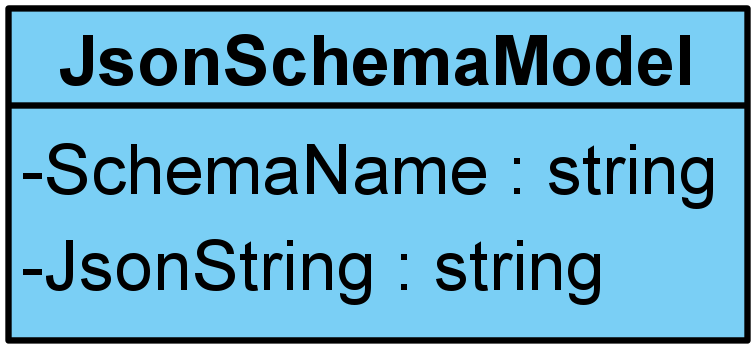
\includegraphics[scale=0.25]{Images/JsonSchemaModel.png}
    \caption{The model of the \texttt{JsonSchema} table.}
    \label{JsonSchemaModel}
\end{figure}
% WordRatio
\begin{figure}[H]
    \centering
    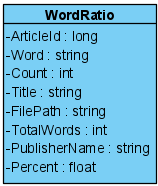
\includegraphics[scale=0.25]{Images/WordRatioModel.png}
    \caption{Diagram of WordRatioModel.}
    \label{WordRatioModel}
\end{figure}


\chapter{SQL script for restoring database structures}\label{SQLBackupScript}
\begin{lstlisting}[
    label=lst:SQLBackupScript,
    language=SQL,
    caption=SQL script for restoring database structures.,
    showspaces=false,
    basicstyle=\ttfamily,
    numbers=left,
    numberstyle=\tiny,
    commentstyle=\color{gray},
    escapechar=|
 ]
 DROP TABLE IF EXISTS "Word" CASCADE;
 DROP TABLE IF EXISTS "Contains" CASCADE;
 DROP TABLE IF EXISTS "Article" CASCADE;
 DROP SEQUENCE IF EXISTS "OccursIn_SEQ" CASCADE;
 DROP SEQUENCE IF EXISTS "Article_Id_seq" CASCADE;
 DROP TABLE IF EXISTS "OccursIn";
 
 ALTER TABLE IF EXISTS "Article_Redundant"
     RENAME TO "Article";
 
 ALTER TABLE IF EXISTS "Term_Redundant"
     RENAME TO "Term";
 
 DROP VIEW "WordRatio";
 CREATE VIEW "WordRatio" AS
 SELECT "ArticleId", "Word", "Count", "Title", "FilePath", "TotalWords","Article"."PublisherName",
        round("Count"::numeric / "TotalWords"::numeric * 100::numeric, 2) AS "Percent"
 FROM "Article"
          JOIN "Term" ON "ArticleId" = "Article"."Id"
          JOIN "Publisher" ON "Article"."PublisherName" = "Publisher"."PublisherName";
\end{lstlisting}